\chapter{Development}

\label{ch:conclusions}

\section{Introduction}

As explained in the design chapter, this project includes three deliverables. So the development will include; a Mac app dashboard, Perfect web-server and CocoaPods framework. Using the "tree-shaped" methodology the web-server was split up into their separate sections which include development, testing, and run. Then each service was design, developed and testing before moving up the tree. The development then broken up into phases, this way the project can be kept on track on what has been completed and whats left to do.

\begin{enumerate}
  \item Services Development
  \item Integrate into Live App
  \item Dashboard Development
  \item CocoaPod Framework 
\end{enumerate}

\section{Project Management}

Good software project management is essential in developing and delivery of software projects. Software development is often difficult to estimate the time required to complete the project, especially when using new technologies. Project milestones can be used to monitor the development progress of the project at certain key points. Above includes the list of the key points within the project. Each point had its own time frame; this kind of project can lead to expanding to including more services and tools, so sticking to the list will help be on schedule.

This project differs from commercial project, in that the project manager, designer, developer and tester were all the same person. And with any project, testing plays a major role in software development and can easily be left out. So self-discipline was required as there was no "boss" to answer to. 

\section{Services Development}

Each service had it's own Perfect server application along with Playground app. This made is easy to decide whether or not it was possible to implement each service into the project. For some of the services, the same Perfect web-server was used and able to be adapted to accommodate the requests needed. 

\paragraph{Setup} Before any development was started, some services was required to be setup. Perfect web-server developers provides an "assistant" to help with the setup and include and required packages needed to develop the API. The list of packages for the project include the following:

\begin{enumerate}
  \item https://github.com/PerfectlySoft/Perfect-Turnstile-MongoDB.git
  
  -Used to provide functionality to interact with MongoDB database, and provide authentication when requests come to the server.
  \item https://github.com/PerfectlySoft/Perfect-RequestLogger.git
  
  -Provides the web-server with a logging system.
  \item https://github.com/hkellaway/Gloss.git
  \item https://github.com/PerfectlySoft/Perfect-Notifications.git
  
  -Aid with the push notifications.
  \item https://github.com/PerfectlySoft/Perfect-SMTP.git
  
  -To be able to send Mails
  \item https://github.com/PerfectlySoft/Perfect-Zip.git
  
  -To zip backups folders, when sending to remote location.
\end{enumerate}

\newpage

After the Perfect web-server was setup, the mongoDB was required to installed locally. This was done by running the following commands in list \ref{lst:mongodb}

\lstinputlisting[label={lst:mongodb}, language=Bash, caption=MongoDB setup]{development/code/mongo.m}


\lstinputlisting[label={lst:playground},language=Swift, caption=Playgrounds setup]{development/code/playground.m}

To be able to run asynchronous code in the playgrounds, the following lines of code in list \ref{lst:playground} is required to be added to the top of the file. This will to make asynchronous code and get results.

\subsubsection{Database storage}

The database storage required an object role model (ORM) which is a powerful method for designing and querying database models at the conceptual level, where the application is described in terms easily understood by non-technical database developers. It is a technique for converting data between incompatible type systems in object-oriented programming languages. The ORM was developed using Playground tool, where the creation of objects and parsing into JSON objects. The functionality of the ORM is to create a new object, parse it and send to the server, and be able to bring all objects back from the server. Extra functionality was added to be able to send filters.

\begin{figure}[!h]
    \caption{Storage Sequence Standard}
    \centering
    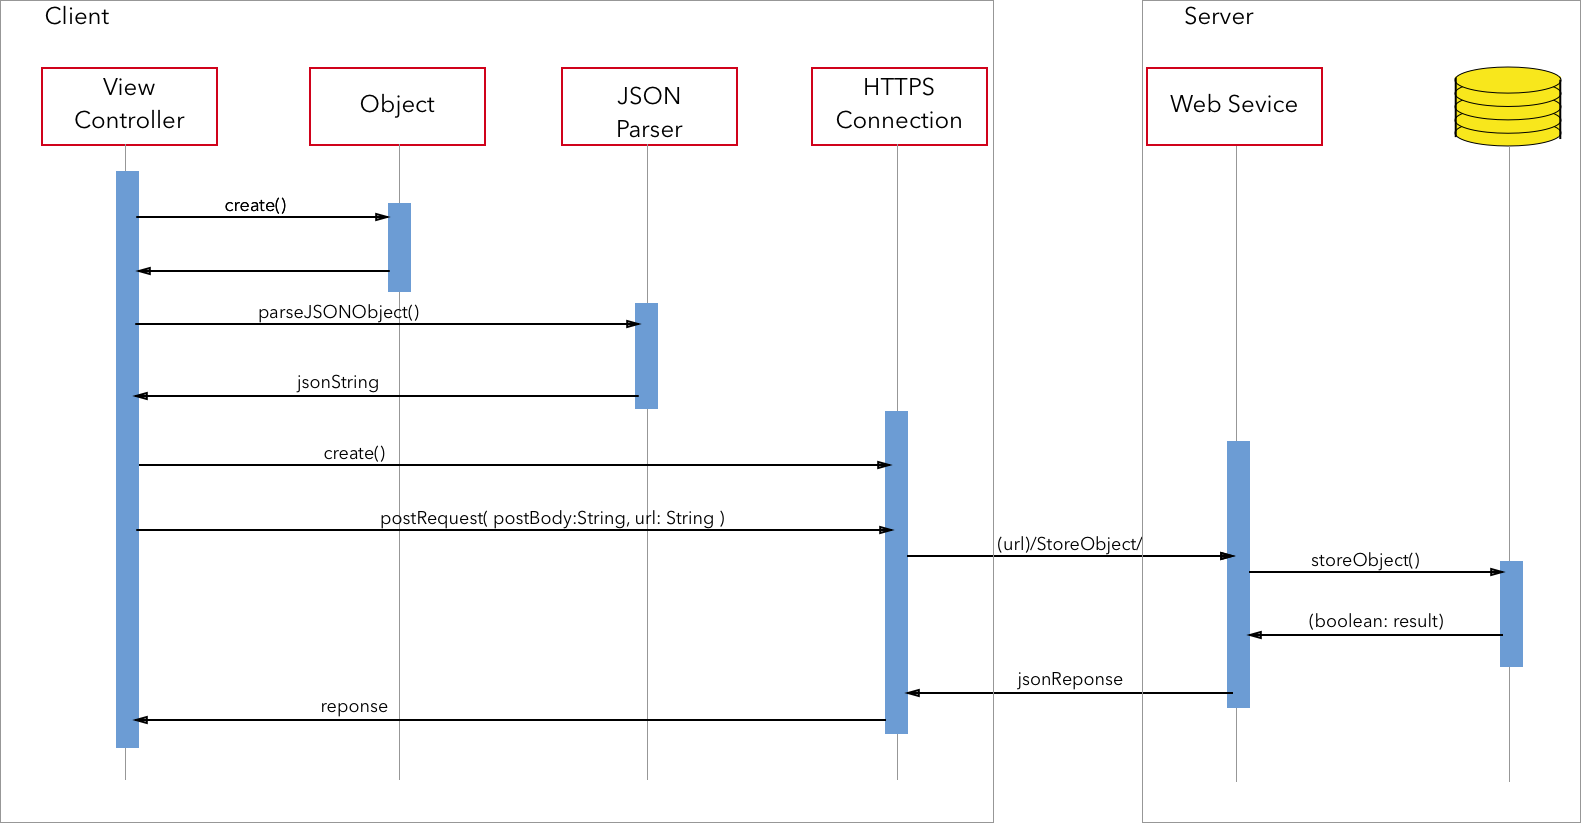
\includegraphics[width=100mm]{images/services/storage_sequence_current}
    \label{fig:storage_old}
\end{figure}


\begin{figure}[!h]
    \caption{Storage Sequence New}
    \centering
    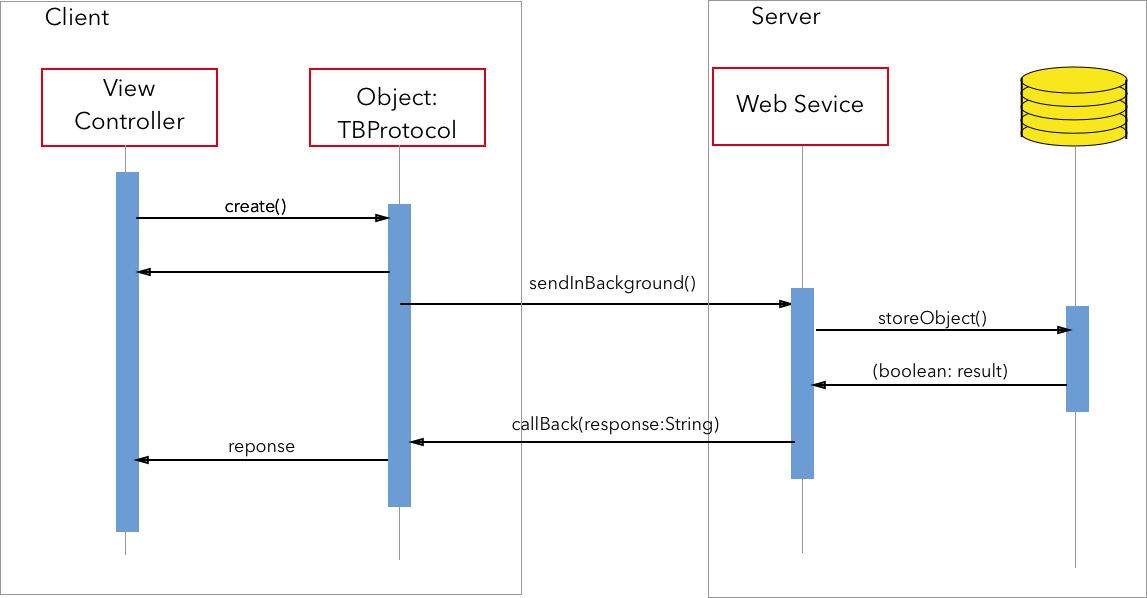
\includegraphics[width=100mm]{images/services/storage_sequence}
    \label{fig:storage_new}
\end{figure}

The two figures above show the difference to developing the standard way, with the developing having to create a JSON parser and then set-up a HTTPS connection to send it to the server in Fig \ref{fig:storage_old} . The new way in Fig \ref{fig:storage_new} using the project's storage protocol involves the developer only having to create the object, then using the objects functionality to send it to the server.

\subsubsection{Apple Push Notifications (APNs)}

Push notifications requires a number of steps to be implemented. First the .p8 key was downloaded, then the Perfect server test project required accessing that file to send notifications. Using the DIT-Timetable app to receive the push notifications.  

\begin{figure}[!h]
    \caption{APNs \cite{apns}}
    \centering
    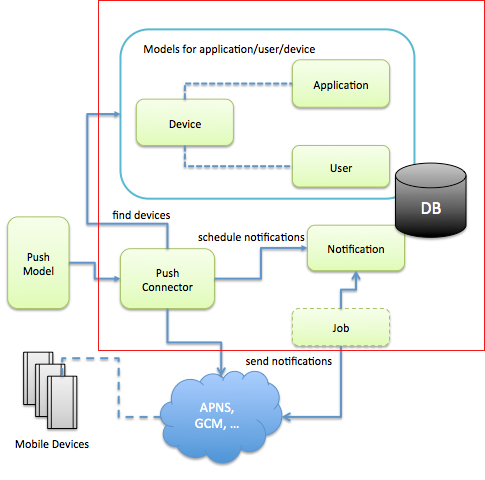
\includegraphics[width=75mm]{images/APNs}
    \label{fig:apns}
\end{figure}

In fig \ref{fig:apns} represents the stages in which to send push notifications. Inside the red box is the server layer, where the .p8 file is located, the push model is where the messages come from. The notifications goes through Apple's sandbox APNs, then on to the mobile devices.


\subsubsection{Analytics}

\paragraph{Level 1}
The first part for the analytic developed was the creation of the Perfect web-server which excepted POST requests. A playground application was developed with the lines of code in list \ref{lst:playground} to aid with HTTP requests. This class made gathers some information before sending the request, this include, time-stamp, build version, OS version, device make and model. For the purposes of testing this service, the data was hard-coded in separate function, that in turn would be reading from plist file. Some of methods and the parameters are included in the following table \ref{table:mob_analytics} shows how to use the library to send analytics. The server stores the analytic objects in the database corresponding to the application, this is done using the appKey which is sent up in the API request.

\begin{table}[!h]
\centering
\caption{Analytics Library}
\label{table:mob_analytics}
\begin{tabular}{|c|c|c|c|}
\hline
\rowcolor{green!20}
Library Method                    & Description                        & Parameters    & Result              \\ 
\hline
TBAnalytics.sendOpenApp();        & \makecell{Sends up object\\ with open app type} &   \makecell{view: UIView , \\ method: String? = \#function \\ , file: String? = \#file } & Successful/ Error   \\ 
\hline
TBAnayltics.send();               & \makecell{Send up object \\ with type as option} &  \makecell{ app: UIResponder, \\ type: SendType \\ , method: String? = \#function ,  \\ file: String? = \#file } & Successful/ Error   \\ 
\hline
 \makecell{ TBAnayltics \\.getAllInBackground(); } & \makecell{Retrieves all \\ TBAnayltic objects }   & NONE        & Array of TBAnayltics \\ 
\hline
\end{tabular}%
\end{table}

Fig \ref{table:analytics} shows how to use the API requests outside of the library.

\begin{table}[!h]
\centering
\caption{Analytics API Requests}
\label{table:analytics}
\begin{tabular}{|l|l|l|l|}
\hline
\rowcolor{green!20}
API Call                        & HTTP Method & Description                    & Parameters   \\ \hline
/\{appKey\}/storage/TBAnalytics & POST        & Uploads analytics object       & JSON Object  \\ \hline
/\{appKey\}/storage/TBAnalytics & GET         & Retrieves all analytic objects & JSON Objects \\ \hline
\end{tabular}
\end{table}


\subsubsection{Backup}


\subsubsection{Self hosted}


\subsubsection{Remote Configuration}


\subsubsection{A/B Testing}


\subsubsection{Live Database}


\subsubsection{Exception catching}


\section{Integrate into Live App}

For some parts of project, an already developed and published app called DIT-Timetable was used to add in the services, to test if Apple would allow it through. The services include remote configuration and language choice. Due to Apple's strict guidelines, the remote configuration was developed into the DIT-Timetable app into two stages, then each stage had a build and published.

\subsubsection{Phase 1}
This phase included just the basic remote configuration, with the capability of updating text such as page title, and label values. Apple did approve this phase, and while the app live, using the iPad prototyping app the text values were able to be changed. 

\subsubsection{Phase 2}

Phase 2 gave the ability to adjust user interface values such as text colour, text size and user interaction enabling/disabling. This also been approved by Apple giving it a go ahead to be completely integrated into the project.  

\section{Dashboard Development}

The dashboard was originally going to be created as an iPad app, but after some thought that not all mobile developers can be expected to own an iPad, the dashboard was developed as a Mac App. 

\section{CocoaPod Framework}

The CocoaPod was left to last to development, as all the test cases used in the Playground could be brought over and adjusted to fit the framework. After the CocoaPod was finished, a test project was created for external professional mobile developers to use and give some feedback.